\documentclass[aspectratio=169,11pt]{beamer}

\usefonttheme{professionalfonts}
\usepackage[T1]{fontenc}
\usepackage[utf8]{inputenc}
\usepackage{lmodern}
\renewcommand{\familydefault}{\sfdefault}
\usepackage{amsmath,amssymb}
\usepackage{booktabs}
\usepackage{array}
\usepackage{graphicx}
\usepackage{tikz}
\usetikzlibrary{calc,positioning,arrows.meta}
\usepackage{ragged2e}

\setbeamertemplate{navigation symbols}{}
\setbeamertemplate{headline}{}
\setbeamertemplate{blocks}[rounded][shadow=false]

\definecolor{TuringInk}{RGB}{22,24,26}
\definecolor{TuringBlue}{RGB}{62,102,163}
\definecolor{TuringSky}{RGB}{143,182,220}
\definecolor{TuringCream}{RGB}{251,249,244}
\definecolor{TuringPanel}{RGB}{241,236,228}
\definecolor{TuringFog}{RGB}{223,217,208}
\definecolor{TuringMuted}{RGB}{112,104,94}
\definecolor{TuringLine}{RGB}{205,198,188}

\setbeamercolor{normal text}{fg=TuringInk,bg=TuringCream}
\setbeamercolor{background canvas}{bg=TuringCream}
\setbeamercolor{structure}{fg=TuringBlue}
\setbeamercolor{title}{fg=TuringInk}
\setbeamercolor{subtitle}{fg=TuringMuted}
\setbeamercolor{frametitle}{fg=TuringInk,bg=TuringCream}
\setbeamercolor{block title}{fg=TuringInk,bg=TuringPanel}
\setbeamercolor{block body}{fg=TuringInk,bg=TuringPanel!75!white}
\setbeamercolor{item}{fg=TuringBlue}

\setbeamerfont{title}{size=\fontsize{24}{28}\selectfont,series=\bfseries}
\setbeamerfont{subtitle}{size=\large}
\setbeamerfont{frametitle}{size=\LARGE,series=\bfseries}
\setbeamerfont{block title}{series=\bfseries}

\setbeamertemplate{frametitle}{%
  \vspace{0.4em}
  \begin{beamercolorbox}[wd=\paperwidth,leftskip=1.1cm,rightskip=1.1cm,sep=0.2cm]{frametitle}
    \usebeamerfont{frametitle}\insertframetitle
  \end{beamercolorbox}
}

\setbeamertemplate{footline}{%
  \leavevmode%
  \hbox{%
    \begin{beamercolorbox}[wd=.82\paperwidth,ht=2.8ex,dp=1.2ex,leftskip=1.05cm]{author in head/foot}%
    \end{beamercolorbox}%
    \begin{beamercolorbox}[wd=.18\paperwidth,ht=2.8ex,dp=1.2ex,rightskip=1.05cm plus1fil]{date in head/foot}%
      \color{TuringMuted}\scriptsize \insertframenumber
    \end{beamercolorbox}}%
}

\title{Diffusion Processing Unit}
\subtitle{The silicon wedge for always-on generative inference}
\author{Turing}
\date{October 2026}

\newcommand{\money}[1]{\$#1}

\newcommand{\marketpie}[4]{%
\begin{tikzpicture}[scale=0.9]
  \def\r{1.25}
  \def\rin{0.58}
  \pgfmathsetmacro{\ang}{#1/100*360}
  \fill[TuringBlue] (0,0) -- (90:\r) arc[start angle=90,end angle=90-\ang,radius=\r] -- cycle;
  \fill[TuringFog] (0,0) -- (90-\ang:\r) arc[start angle=90-\ang,end angle=-270,radius=\r] -- cycle;
  \fill[TuringCream] (0,0) circle (\rin);
  \draw[TuringLine,line width=0.8pt] (0,0) circle (\r);
  \node[font=\bfseries\large] at (0,0.05) {#2};
  \node[align=center,font=\scriptsize,text=TuringMuted] at (0,-1.65) {#3};
  \node[align=center,font=\tiny,text=TuringMuted] at (0,-2.0) {#4};
\end{tikzpicture}%
}

\newcommand{\softpanel}[2]{%
\begin{beamercolorbox}[wd=\linewidth,sep=0.8em,rounded=true]{block body}
{\bfseries #1}\\[0.25em]
{\small #2}
\end{beamercolorbox}
}

\begin{document}

\begin{frame}[plain]
  \vspace{1.4em}
  {\color{TuringMuted}\large Turing}

  \vspace{0.5em}

  {\usebeamerfont{title}\inserttitle\par}

  \vspace{0.45em}
  {\usebeamerfont{subtitle}\color{TuringMuted}\insertsubtitle\par}

  \vspace{0.9em}

  \begin{columns}[T,totalwidth=\textwidth]
    \begin{column}{0.53\textwidth}
      \begin{beamercolorbox}[wd=\linewidth,sep=1.0em,rounded=true]{block body}
        \large Stable Diffusion made image generation feel like a real product category almost overnight. The next question is how to serve that demand---and the wave of video that follows---without paying GPU economics forever. Open models moved generative media from demo to daily use.
      \end{beamercolorbox}
    \end{column}
    \begin{column}{0.43\textwidth}
      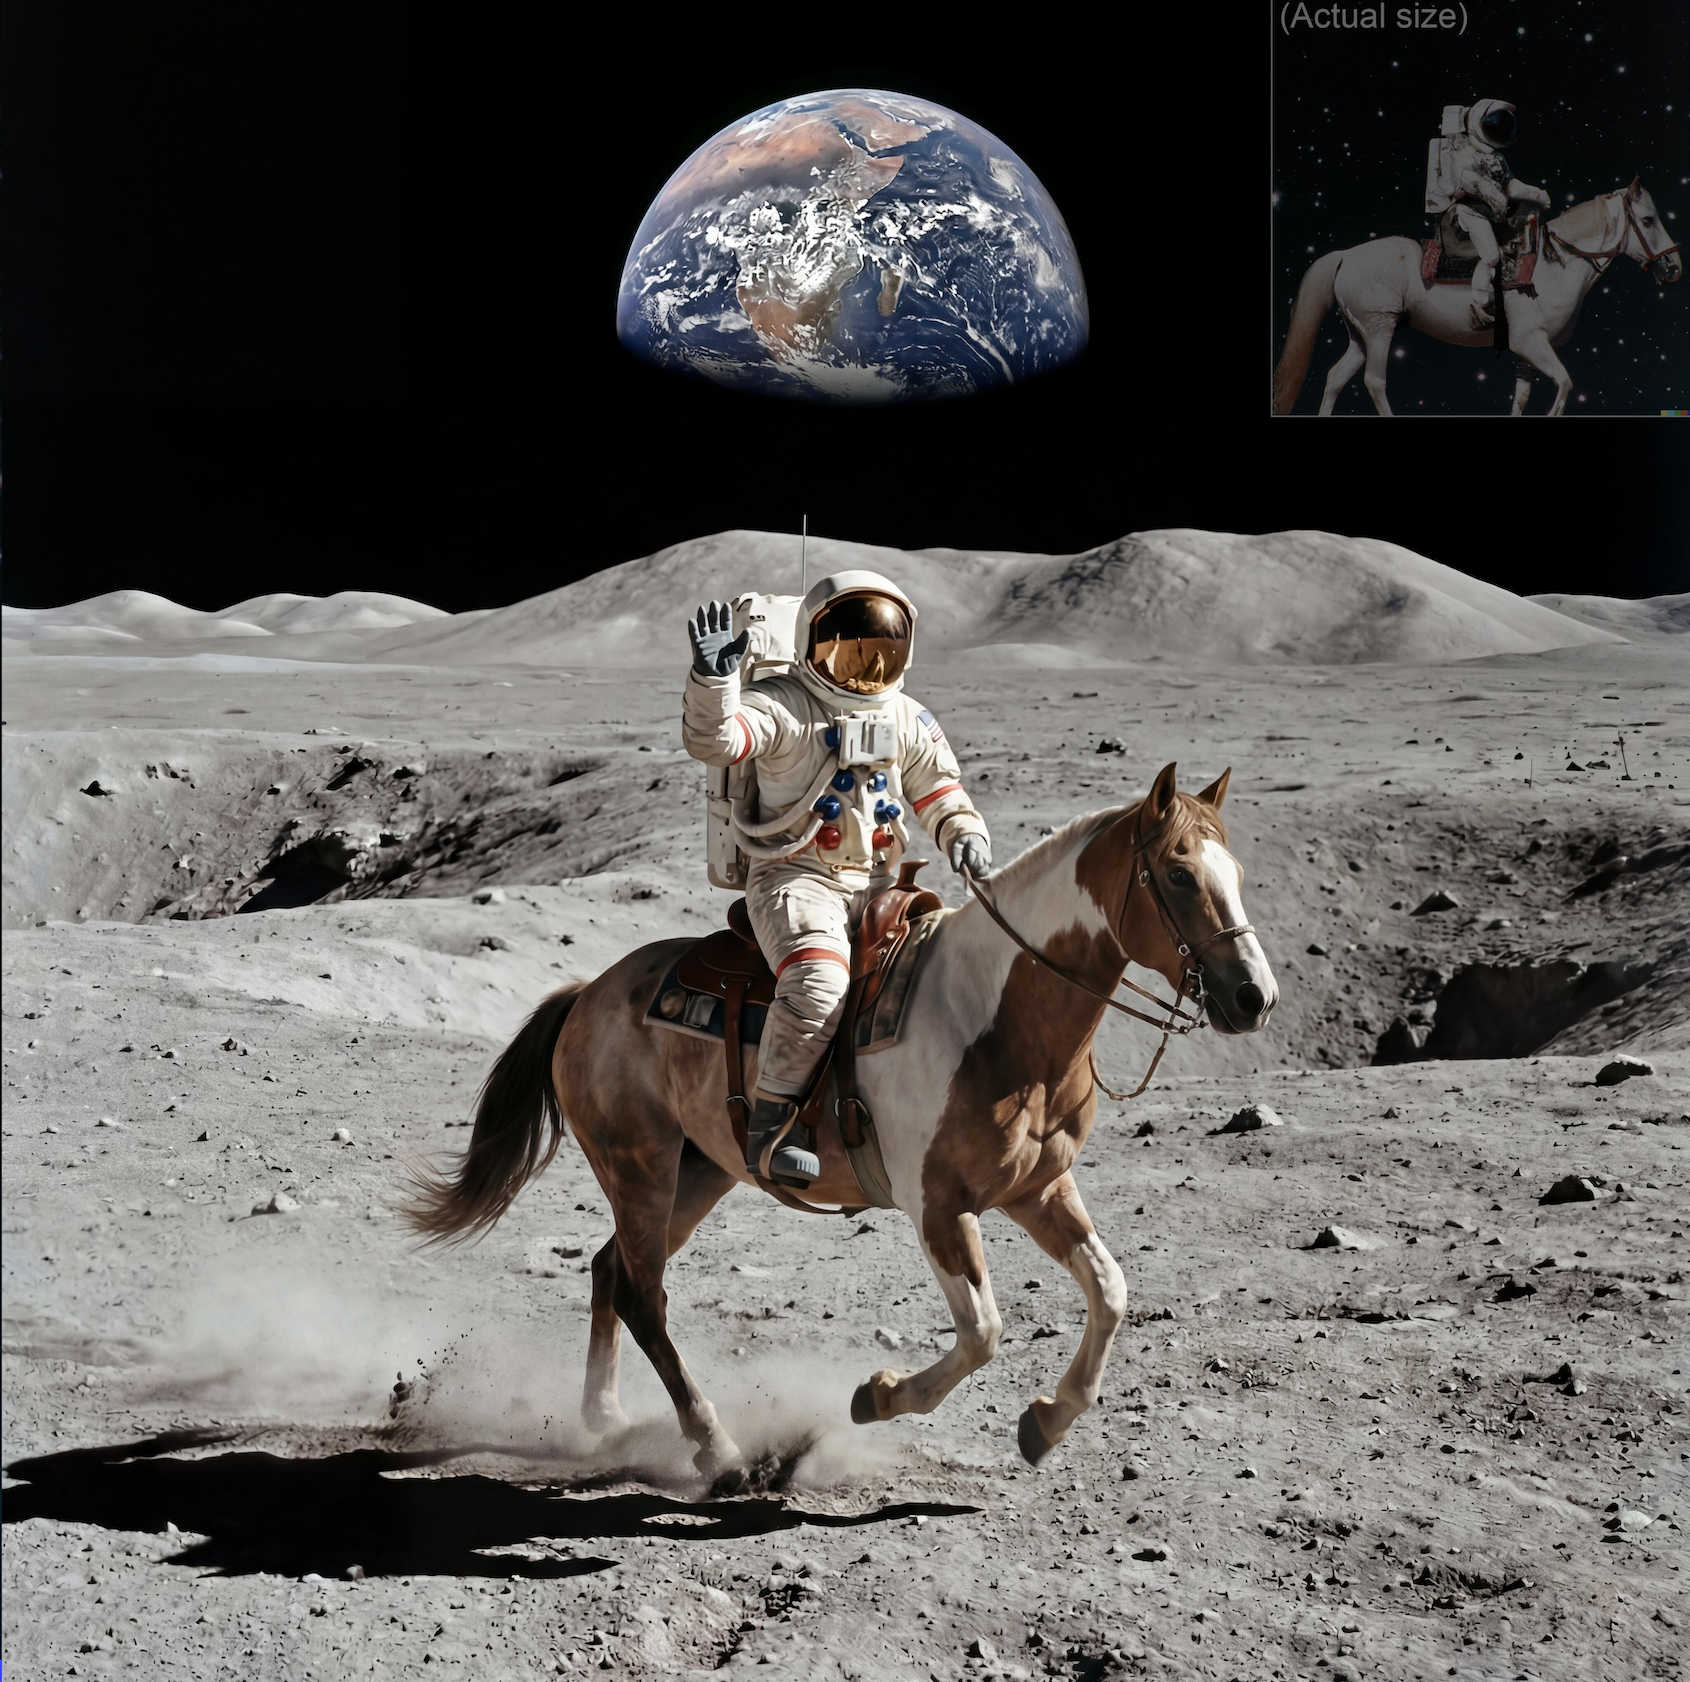
\includegraphics[width=\linewidth,height=0.64\textheight,keepaspectratio]{diffusion.png}
    \end{column}
  \end{columns}
\end{frame}

\begin{frame}{Demand is already here, and it is widening}
\begin{columns}[T,totalwidth=\textwidth]
  \begin{column}{0.68\textwidth}
    \begin{beamercolorbox}[wd=\linewidth,sep=0.9em,rounded=true]{block body}
      \begin{center}
      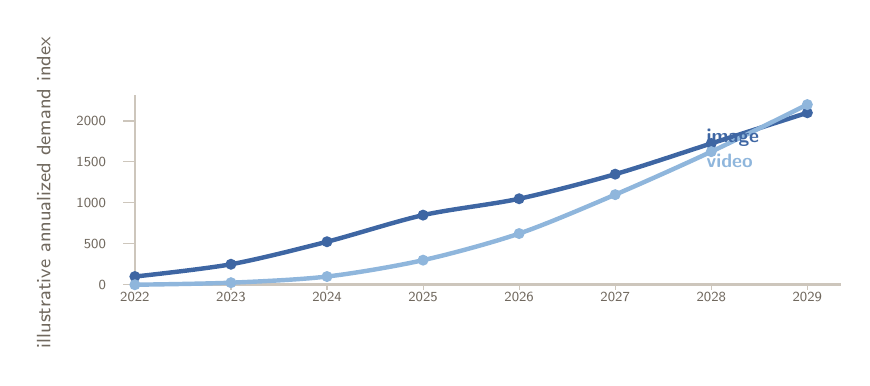
\begin{tikzpicture}[x=1.22cm,y=0.13cm]
        \draw[TuringLine,line width=0.9pt] (0,0) -- (7.35,0);
        \draw[TuringLine,line width=0.9pt] (0,0) -- (0,18.5);

        \foreach \x/\yr in {0/2022,1/2023,2/2024,3/2025,4/2026,5/2027,6/2028,7/2029} {
          \draw[TuringLine] (\x,0) -- (\x,-0.5);
          \node[font=\tiny,text=TuringMuted] at (\x,-1.15) {\yr};
        }

        \foreach \y/\label in {0/0,4/500,8/1000,12/1500,16/2000} {
          \draw[TuringLine] (0,\y) -- (-0.12,\y);
          \node[font=\tiny,text=TuringMuted,anchor=east] at (-0.2,\y) {\label};
        }

        \node[font=\scriptsize,text=TuringMuted,rotate=90] at (-0.95,9) {illustrative annualized demand index};

        \draw[TuringBlue,line width=1.6pt] plot[smooth] coordinates {(0,0.8) (1,2.0) (2,4.2) (3,6.8) (4,8.4) (5,10.8) (6,13.8) (7,16.8)};
        \foreach \x/\y in {0/0.8,1/2.0,2/4.2,3/6.8,4/8.4,5/10.8,6/13.8,7/16.8} {
          \fill[TuringBlue] (\x,\y) circle (2pt);
        }

        \draw[TuringSky,line width=1.6pt] plot[smooth] coordinates {(0,0.0) (1,0.2) (2,0.8) (3,2.4) (4,5.0) (5,8.8) (6,13.0) (7,17.6)};
        \foreach \x/\y in {0/0.0,1/0.2,2/0.8,3/2.4,4/5.0,5/8.8,6/13.0,7/17.6} {
          \fill[TuringSky] (\x,\y) circle (2pt);
        }

        \node[font=\scriptsize\bfseries,text=TuringBlue,anchor=west] at (5.85,14.4) {image};
        \node[font=\scriptsize\bfseries,text=TuringSky,anchor=west] at (5.85,12.1) {video};
      \end{tikzpicture}
      \end{center}
    \end{beamercolorbox}
  \end{column}
  \begin{column}{0.30\textwidth}
    \begin{beamercolorbox}[wd=\linewidth,sep=0.8em,rounded=true]{block body}
      {\bfseries Demand snapshot}\\[0.35em]
      {\small \textbf{2026E}\\Image index: \textbf{1,050}\\Video index: \textbf{625}}\\[0.55em]
      {\small \textbf{2029E}\\Image index: \textbf{2,100}\\Video index: \textbf{2,200}}\\[0.55em]
      {\scriptsize Indexed to Stable Diffusion-era image adoption. Directional operating-demand view only.}
    \end{beamercolorbox}
  \end{column}
\end{columns}
\end{frame}

\begin{frame}{Image first, video close behind}
\begin{columns}[T,totalwidth=\textwidth]
  \begin{column}{0.55\textwidth}
    \begin{itemize}
      \item Text-to-image proved the commercial habit. Video compounds the same diffusion logic across far more frames, so its infrastructure curve should steepen quickly.
      \item That makes this an image market now and a video market soon after---with enough architectural overlap to target both from the beginning.
      \item Once usage is continuous, the buying question becomes simple: how many outputs can a rack produce, at what margin, and at what power draw?
    \end{itemize}
  \end{column}
  \begin{column}{0.45\textwidth}
    \softpanel{What customers feel}{\money{15--40} per 1{,}000 diffusion inferences is tolerable for experimentation and painful for scaled, always-on deployment.}

    \vspace{0.7em}

    \softpanel{What specialized silicon offers}{A 5--20$\times$ lower inference-cost target and a 10--50$\times$ power advantage on the denoising path, before video demand widens the gap further.}
  \end{column}
\end{columns}
\end{frame}

\begin{frame}{Why a DPU wins this wedge}
\begin{columns}[T,totalwidth=\textwidth]
  \begin{column}{0.34\textwidth}
    \begin{beamercolorbox}[wd=\linewidth,sep=1em,rounded=true]{block body}
      {\bfseries Fixed loop, not general theater}

      \vspace{0.35em}
      \small Diffusion inference repeats a denoising pattern often enough to justify hardware that is priced for the loop, not for every possible model path.
    \end{beamercolorbox}
  \end{column}
  \begin{column}{0.33\textwidth}
    \begin{beamercolorbox}[wd=\linewidth,sep=1em,rounded=true]{block body}
      {\bfseries Tile first, system second}

      \vspace{0.35em}
      \small A narrow signed-int8 MAC tile already maps to convolution, attention, and MLP-heavy denoising kernels.
    \end{beamercolorbox}
  \end{column}
  \begin{column}{0.33\textwidth}
    \begin{beamercolorbox}[wd=\linewidth,sep=1em,rounded=true]{block body}
      {\bfseries Lower variance matters}

      \vspace{0.35em}
      \small Paid generation services care about predictable latency, stable thermals, and more images per rack as much as headline TOPS.
    \end{beamercolorbox}
  \end{column}
\end{columns}

\vspace{0.9em}

\begin{center}
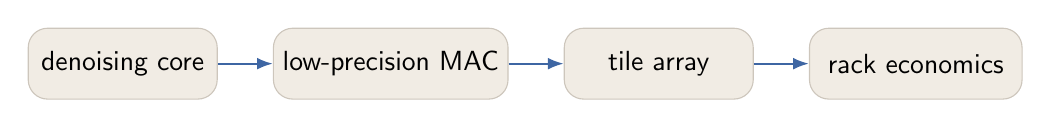
\begin{tikzpicture}[node distance=0.7cm]
  \node[draw=TuringLine,fill=TuringPanel,rounded corners=7pt,minimum width=2.4cm,minimum height=0.9cm] (a) {denoising core};
  \node[draw=TuringLine,fill=TuringPanel,rounded corners=7pt,minimum width=2.4cm,minimum height=0.9cm,right=of a] (b) {low-precision MAC};
  \node[draw=TuringLine,fill=TuringPanel,rounded corners=7pt,minimum width=2.4cm,minimum height=0.9cm,right=of b] (c) {tile array};
  \node[draw=TuringLine,fill=TuringPanel,rounded corners=7pt,minimum width=2.7cm,minimum height=0.9cm,right=of c] (d) {rack economics};
  \draw[-{Latex[length=2mm]},thick,TuringBlue] (a) -- (b);
  \draw[-{Latex[length=2mm]},thick,TuringBlue] (b) -- (c);
  \draw[-{Latex[length=2mm]},thick,TuringBlue] (c) -- (d);
\end{tikzpicture}
\end{center}
\end{frame}

\begin{frame}{Market capture is a wedge story, not a winner-take-all story}
\begin{center}
\begin{columns}[T,totalwidth=0.96\textwidth]
  \begin{column}{0.33\textwidth}
    \centering
    \marketpie{100}{TAM}{AI inference accelerator market}{\money{25B--40B}}
  \end{column}
  \begin{column}{0.33\textwidth}
    \centering
    \marketpie{18}{SAM}{Diffusion-heavy deployment wedge}{\money{3B--8B}}
  \end{column}
  \begin{column}{0.33\textwidth}
    \centering
    \marketpie{3}{SOM}{Early meaningful capture}{\money{50M--250M}+}
  \end{column}
\end{columns}
\end{center}

\vspace{0.7em}

\begin{beamercolorbox}[wd=\textwidth,sep=0.8em,rounded=true]{block body}
\small This is a focused play for the part of inference where image and video generation are persistent enough to justify specialized economics.
\end{beamercolorbox}
\end{frame}

\begin{frame}{Competition is broad. The advantage is narrow and commercial.}
\begin{columns}[T,totalwidth=\textwidth]
  \begin{column}{0.24\textwidth}
    \softpanel{Cloud GPUs}{Great default. Expensive once denoising becomes a margin business.}
  \end{column}
  \begin{column}{0.24\textwidth}
    \softpanel{Hyperscaler silicon}{Powerful, but built for broad internal fleets, not an open wedge.}
  \end{column}
  \begin{column}{0.24\textwidth}
    \softpanel{AI chip startups}{Many chase general AI acceleration. Few stay disciplined on diffusion economics.}
  \end{column}
  \begin{column}{0.24\textwidth}
    \softpanel{CPU / edge fallback}{Cheap to start, poor at sustained commercial throughput.}
  \end{column}
\end{columns}

\vspace{0.9em}

\begin{beamercolorbox}[wd=\textwidth,sep=0.9em,rounded=true]{block body}
\large Turing: better economics for a repeating diffusion workload, with a cleaner path to trustworthy silicon.
\end{beamercolorbox}
\end{frame}

\begin{frame}{Turing's edge: formal verification is a tape-out advantage}
\begin{columns}[T,totalwidth=\textwidth]
  \begin{column}{0.36\textwidth}
    \softpanel{Start small, prove early}{The repository begins with a formally tractable tile: signed int8 arithmetic, saturating accumulation, and explicit valid/ready boundaries.}
  \end{column}
  \begin{column}{0.32\textwidth}
    \softpanel{Cut late surprises}{Protocol bugs and arithmetic edge cases are cheap in RTL and expensive in signoff. Proof moves that pain earlier.}
  \end{column}
  \begin{column}{0.32\textwidth}
    \softpanel{Sell trust, not only speed}{Operators buy confidence that the board, module, and software path will integrate without a long tail of avoidable defects.}
  \end{column}
\end{columns}

\vspace{1em}

\begin{center}
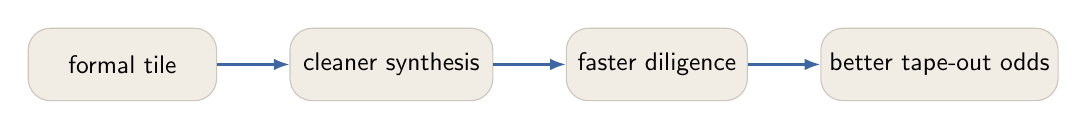
\begin{tikzpicture}[scale=0.92, transform shape]
  \node[draw=TuringLine,fill=TuringPanel,rounded corners=8pt,minimum width=2.6cm,minimum height=1cm] (a) {formal tile};
  \node[draw=TuringLine,fill=TuringPanel,rounded corners=8pt,minimum width=2.8cm,minimum height=1cm,right=1.0cm of a] (b) {cleaner synthesis};
  \node[draw=TuringLine,fill=TuringPanel,rounded corners=8pt,minimum width=2.5cm,minimum height=1cm,right=1.0cm of b] (c) {faster diligence};
  \node[draw=TuringLine,fill=TuringPanel,rounded corners=8pt,minimum width=2.3cm,minimum height=1cm,right=1.0cm of c] (d) {better tape-out odds};
  \draw[-{Latex[length=2mm]},thick,TuringBlue] (a) -- (b);
  \draw[-{Latex[length=2mm]},thick,TuringBlue] (b) -- (c);
  \draw[-{Latex[length=2mm]},thick,TuringBlue] (c) -- (d);
\end{tikzpicture}
\end{center}
\end{frame}

\begin{frame}{Go-to-market: partner with Southern U.S. AI buildouts}
\begin{columns}[T,totalwidth=\textwidth]
  \begin{column}{0.5\textwidth}
    \begin{itemize}
      \item New AI capacity is easier to shape than installed GPU fleets are to displace.
      \item Southern buildouts offer power, land, cooling expansion, and procurement flexibility.
      \item The pitch: more generated output per watt, per rack, and per megawatt committed to generative media.
    \end{itemize}
  \end{column}
  \begin{column}{0.5\textwidth}
    \softpanel{Target profiles, not yet named deals}{Texas, Tennessee, and Georgia are attractive because new AI halls are often planned in 20--100+ MW increments, where accelerator choice still affects the economics of the build.}
  \end{column}
\end{columns}

\vspace{0.5em}

\begin{columns}[T,totalwidth=\textwidth]
  \begin{column}{0.32\textwidth}
    \begin{beamercolorbox}[wd=\linewidth,sep=0.65em,rounded=true]{block body}
      {\bfseries Pod pilot}\\[0.2em]
      {\scriptsize 20 MW-class pod\\design partner + trial}
    \end{beamercolorbox}
  \end{column}
  \begin{column}{0.32\textwidth}
    \begin{beamercolorbox}[wd=\linewidth,sep=0.65em,rounded=true]{block body}
      {\bfseries Regional AI hall}\\[0.2em]
      {\scriptsize 50 MW-class cluster\\rack-scale proof}
    \end{beamercolorbox}
  \end{column}
  \begin{column}{0.32\textwidth}
    \begin{beamercolorbox}[wd=\linewidth,sep=0.65em,rounded=true]{block body}
      {\bfseries Campus expansion}\\[0.2em]
      {\scriptsize 100 MW+ buildout\\module standardization}
    \end{beamercolorbox}
  \end{column}
\end{columns}
\end{frame}

\begin{frame}{The next 12 months}
\begin{center}
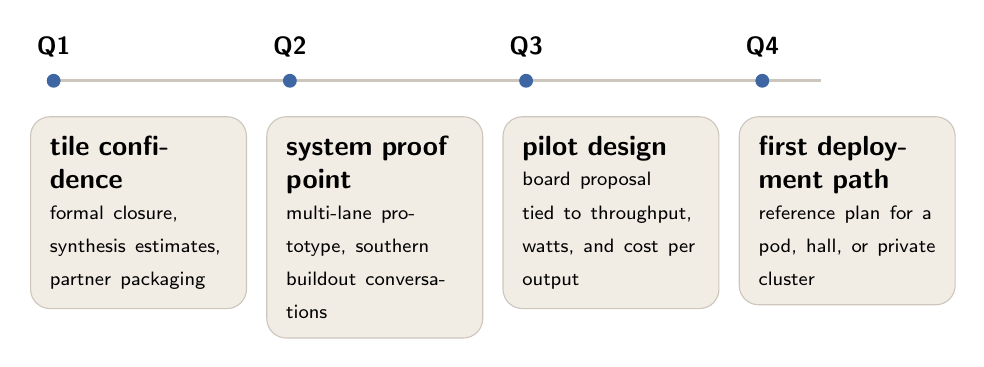
\begin{tikzpicture}[x=3.0cm,y=1cm]
  \draw[TuringLine,line width=1.2pt] (0,0) -- (3.25,0);
  \foreach \x/\q/\title/\desc in {
    0/{Q1}/{tile confidence}/{formal closure, synthesis estimates, partner packaging},
    1/{Q2}/{system proof point}/{multi-lane prototype, southern buildout conversations},
    2/{Q3}/{pilot design}/{board proposal tied to throughput, watts, and cost per output},
    3/{Q4}/{first deployment path}/{reference plan for a pod, hall, or private cluster}
  } {
    \fill[TuringBlue] (\x,0) circle (2.5pt);
    \node[font=\bfseries\small,anchor=south] at (\x,0.18) {\q};
    \node[draw=TuringLine,fill=TuringPanel,rounded corners=7pt,align=left,text width=2.25cm,anchor=north west,inner sep=7pt] at ($(\x,0)+(-0.1,-0.45)$) {\textbf{\title}\\[-0.1em]\scriptsize \desc};
  }
\end{tikzpicture}
\end{center}

\vspace{0.8em}

\begin{beamercolorbox}[wd=\textwidth,sep=0.9em,rounded=true]{block body}
\large The first win is not a global platform. It is one buildout where image and video generation are expensive enough to justify a better chip.
\end{beamercolorbox}
\end{frame}

\begin{frame}[plain]
\vspace{1.4em}
\begin{center}
  {\fontsize{28}{34}\selectfont\bfseries Build for image now. Grow into video fast.}\par

  \vspace{0.8em}
  {\large The same optimization that improves image-generation economics becomes even more valuable as video generation scales.}\par

  \vspace{1.0em}

  \begin{columns}[T,totalwidth=0.96\textwidth]
    \begin{column}{0.32\textwidth}
      \softpanel{Illustrative savings}{At 100M generations per month, a move from \money{25} to \money{5} per 1{,}000 outputs implies roughly \money{24M} in annualized savings.}
    \end{column}
    \begin{column}{0.32\textwidth}
      \softpanel{Why video matters}{Video multiplies denoising demand across time. If image is the first commercial wedge, video is the force that widens it.}
    \end{column}
    \begin{column}{0.32\textwidth}
      \softpanel{Turing's opening}{Win one image-heavy deployment first, but build the architecture and sales story with image-plus-video infrastructure in mind from day one.}
    \end{column}
  \end{columns}

  \vspace{1.0em}

  \begin{beamercolorbox}[wd=0.74\textwidth,sep=0.9em,rounded=true]{block body}
    \centering
    \large Turing\\[0.2em]
    \normalsize formal-verification-first silicon for generative media infrastructure
  \end{beamercolorbox}
\end{center}
\end{frame}

\end{document}


